\begin{figure}[H]
    \centering
    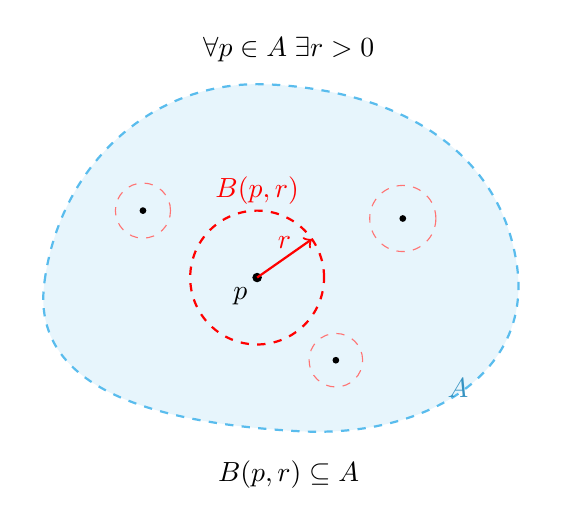
\begin{tikzpicture}[scale=1.0]
        % Conjunto aberto A.
        \path[fill=Cerulean!10]
            (0.0,0.2)
            .. controls (0.2,1.7) and (1.4,2.8) .. (2.9,2.7)
            .. controls (4.6,2.6) and (5.8,1.8) .. (6.0,0.4)
            .. controls (6.2,-1.0) and (4.8,-1.8) .. (3.2,-1.7)
            .. controls (1.5,-1.6) and (-0.2,-1.2) .. (0.0,0.2)
            -- cycle;
        \draw[Cerulean!70, thick, dashed]
            (0.0,0.2)
            .. controls (0.2,1.7) and (1.4,2.8) .. (2.9,2.7)
            .. controls (4.6,2.6) and (5.8,1.8) .. (6.0,0.4)
            .. controls (6.2,-1.0) and (4.8,-1.8) .. (3.2,-1.7)
            .. controls (1.5,-1.6) and (-0.2,-1.2) .. (0.0,0.2)
            -- cycle;

        % Um ponto arbitrario e uma bola aberta contida em A.
        \filldraw[black] (2.7,0.25) circle (1.5pt) node[below left] {$p$};
        \draw[Red, thick, dashed] (2.7,0.25) circle (0.85);
        \draw[Red, thick, ->] (2.7,0.25) -- ++(35:0.85)
            node[midway, above] {$r$};

        % Outros pontos indicam que a condicao vale em todo o conjunto.
        \filldraw[black] (1.25,1.1) circle (1pt);
        \draw[Red!55, dashed] (1.25,1.1) circle (0.35);

        \filldraw[black] (4.55,1.0) circle (1pt);
        \draw[Red!55, dashed] (4.55,1.0) circle (0.42);

        \filldraw[black] (3.7,-0.8) circle (1pt);
        \draw[Red!55, dashed] (3.7,-0.8) circle (0.34);

        \node[Cerulean!80!black] at (5.25,-1.15) {$A$};
        \node[Red] at (2.7,1.35) {$B(p,r)$};
        \node at (3.1,3.15) {$\forall p\in A\;\exists r>0$};
        \node at (3.1,-2.25) {$B(p,r)\subseteq A$};
    \end{tikzpicture}
    \caption{Ilustração da noção de conjunto aberto.}
\end{figure}